% Created 2011-08-22 Mon 11:27
\documentclass[11pt]{article}
%\usepackage[utf8]{inputenc}
\usepackage[T1]{fontenc}
\usepackage{graphicx}
\usepackage{longtable}
\usepackage{hyperref}
\usepackage{comment}
\usepackage{booktabs}
\usepackage{color}
\usepackage{pgf}
\usepackage{tikz}
\usetikzlibrary{arrows,positioning,fit,shapes,decorations,decorations.pathmorphing,decorations.pathreplacing,calc,patterns,scopes,matrix}
\pgfrealjobname{spi}
 
\usepackage{helvet}
\usepackage{enumitem}
\usepackage[letterpaper]{geometry}
\usepackage{listings}
\usepackage{verbatim}
\usepackage[T1]{fontenc}

\setlength{\parindent}{0.0in}
\setlength{\parskip}{0.1in}

\newenvironment{apient}{\small\verbatim}{\endverbatim}

\newcommand{\apidesc}[1]{%
{\addtolength{\leftskip}{4em}%
#1\par\medskip}
}

\begin{document}
\thispagestyle{empty}

\begin{titlepage}
\beginpgfgraphicnamed{titlepage}
\begin{tikzpicture}[remember picture, overlay]
    \path
        (current page.north west) coordinate (origin)
        (current page.north) coordinate (topcenter);

    % Header
    \node [font=\sffamily] (pppt) at ($(topcenter) - (0,1.0in)$) 
        {\fontsize{24}{36}\selectfont Paradyn Parallel Performance Tools};

    % Document Title
% older versions of pgf have a bug for matrices in overlay mode;
% have to specify positions manually
    \matrix (Title) [%
        matrix of nodes,%
        nodes={font=\sffamily,right},%
        matrix anchor=west,%
        row sep=12pt
        ] at ($(origin)+(0.75in,-3.0in)$)
    {
        \fontsize{48}{56}\selectfont Self-propelled Instrumentation \\ \\ \\ \\ \\
        \fontsize{48}{56}\selectfont Developer's Manual \\
    };

    \node [anchor=west,font=\sffamily] (title1) at ($(origin)+(0.75in,-3.0in)$)
        {\fontsize{48}{56}\selectfont };
%    \node [anchor=west,font=\sffamily] (title2) at ($(title1.west)+(0in,-56pt)$)
%        {\fontsize{48}{56}\selectfont Programmer's Guide};

    % Release information
%    \matrix (Releaseinfo) [%
%        matrix of nodes,%
%        nodes={font=\sffamily,right},%
%        matrix anchor=west,%
%        row sep=8pt
%        ] at ($(origin)+(0.75in,-5.0in)$)
%    {
%        %\fontsize{24}{32}\selectfont Release 0.1 \\
%        \fontsize{24}{32}\selectfont Beta Release \\
%        \fontsize{24}{32}\selectfont Oct 2010 \\
%    };

    \node [anchor=west,font=\sffamily] (rel1) at ($(origin)+(0.75in,-5.0in)$)
        {\fontsize{24}{32}\selectfont 1.0b Release};
    \node [anchor=west,font=\sffamily] (rel2) at ($(rel1.west)+(0in,-32pt)$)
        {\fontsize{24}{32}\selectfont September 2012};

    % Contact information
%    \matrix (UWaddress) [%
%        matrix of nodes,%
%        nodes={font=\sffamily\large,right},%
%        matrix anchor=north west
%        ] at ($(origin)+(0.75in,-7in)$)
%    {
%        Computer Science Department \\
%        University of Wisconsin--Madison \\
%        Madison, WI 53711 \\
%    };

    \node [anchor=west,font=\sffamily\large] (uw1) at ($(origin)+(0.75in,-7.0in)$)
        {Computer Science Department};
    \node [anchor=west,font=\sffamily\large] (uw2) at ($(uw1.west)+(0in,-20pt)$)
        {University of Wisconsin--Madison};
    \node [anchor=west,font=\sffamily\large] (uw3) at ($(uw2.west)+(0in,-20pt)$)
        {Madison, WI 53711};


%    \matrix (UMDaddress) [%
%        matrix of nodes,%
%        nodes={font=\sffamily\large,right},%
%        matrix anchor=north west,
%        below=1em of UWaddress.south west
%        ]
%    {
%        Computer Science Department \\
%        University of Maryland \\
%        College Park, MD 20742 \\
%    };

    \node [anchor=west,font=\sffamily\large] (umd1) at ($(uw3.south west)+(0in,-2.5em)$)
        {Computer Science Department};
    \node [anchor=west,font=\sffamily\large] (umd2) at ($(umd1.west)+(0in,-20pt)$)
        {University of Maryland};
    \node [anchor=west,font=\sffamily\large] (umd3) at ($(umd2.west)+(0in,-20pt)$)
        {College Park, MD 20742};

%    \matrix (Emails) [%
%        matrix of nodes,%
%        nodes={font=\sffamily,right},%
%        matrix anchor=north west,%
%        below=1em of UMDaddress.south west,%
%        anchor=base
%        ]
%    {
%        Email & \texttt{bugs@dyninst.org} \\
%        Web & \texttt{www.dyninst.org} \\
%    };

    \node [anchor=west,font=\sffamily] (email1) at ($(umd3.south west)+(-0.5em,-2.5em)$)
        %{Email \texttt{bugs@dyninst.org}};
        {\begin{tabular}{ll}%
         Email & \texttt{bugs@dyninst.org} \\
         Web & \texttt{www.dyinst.org} \\
        \end{tabular}};
        

    % Logo
    \path 
        node (logo) at ($(origin)+(4.0in,-7.0in)$) [%
            anchor=north west]
        {%
            
\includegraphics[width=3.25in]{paradyn_logo}
        }; 


\end{tikzpicture}
\endpgfgraphicnamed
\end{titlepage}

\tableofcontents
\clearpage

\section{Introduction}
\label{sec-intro}

Self-propelled instrumentation is a binary instrumentation technique that
dynamically injects a fragment of code into an application process on
demand.
The instrumentation is inserted ahead of the control flow within the process and
is propagated into other processes, following communication events, crossing
host boundaries, and collecting a distributed function-level trace of the
execution.

Self-propelled instrumentation contains two major components, {\em Agent} and
{\em Injector}.
{\em Agent} is a shared library that automatically inserts and propagates a
piece of payload code at function call events in a running process, where the
payload code contains user-defined logic, such as generating trace data for
later inspection.
The instrumentation would propel itself within the process by following control
flow and across thread boundaries, process boundaries, or even host boundaries
by following communication flow.
{\em Injector} is a process that causes an application process to load the Agent
shared library, where the Injector should have at least the same privilege as
the application process.
Self-propelled instrumentation does binary instrumentation within the
application process's address space, avoiding use of the debugging interfaces
(e.g., Linux ptrace and Windows debug interface) and costly interprocess
communications.
Therefore, self-propelled instrumentation does not add significant overhead to a
process during runtime.

Self-propelled instrumentation can be used in many applications that require low
overhead instrumentation and full automation of instrumentation propagation
following control flow.
For example, we have used self-propelled instrumentation for problem diagnosis
in distributed systems~\cite{Mirgorodskiy2006} and for automated diagram
construction for complex software systems in security analysis~\cite{Fang2012}.

\section{Abstraction}
Self-propelled instrumentation has two major components, {\em Agent} that is a
shared library injected into an application process's address space, and {\em
  Injector} that injects {\em Agent}.
The following subsections describe the lower level components in Agent and
Injector in details.

\subsection{Agent}

\begin{itemize}
\item \textbf{Agent}. It manages the configuration and does instrumentation. An
  Agent instance is created in the init function of the {\em Agent} shared
  library.
\item \textbf{Event}. It specifies when the initial instrumentation should be
  done after the {\em Agent} shared library is loaded.  Currently, there are
  four types of Event: 1) instrumenting all callees in {\em main} function right
  away; 2) instrumenting all callees of specified functions right away; 3)
  instrumenting specified function calls right away; 4) instrumenting all
  callees in {\em main} after a given amount of time.
\item \textbf{Payload function}. It contains user-specified code.  From user's
  perspective, a payload function will be invoke before or after each function
  call in the process.  There are two types of payload functions, {\em entry
    payload} that is invoked before each function call and {\em exit payload}
  that is invoked after each function call.
\item \textbf{Point}. It represents an instrumentation point at current function
  call and is used in Payload function.
\item \textbf{Control Flow Graph (CFG) structures}. CFG structures include
  Object, Function, Block, and Edge. An Object represents a binary file (i.e.,
  an executable or a shared library), and contains a set of functions. A
  Function contains a set of Blocks. A Block is a basic block. An Edge connects
  two Blocks. Users can get related CFG structures of current function call from
  Point.
\end{itemize}

 



\subsection{Injector}
% For user / developer manual
% Two types of injection: process start and hijack

Injector is provided as a command. 
There are two types of injections.
One is to inject the {\em Agent} shared library at the very beginning of a
process.
The other is to inject the {\em Agent} in the middle of a running process.

% For developer manual
% Two types of injection: process start and hijack
The first type of Injector relies on dynamic linker (i.e., setting the
environment variable LD\_PRELOAD to the path of an {\em Agent} shared library).
The second type uses ProcControlAPI to force an application process to invoke
functions in the dlopen family.



\section{How it works}
This section describes how self-propelled instrumentation works in details.
Each subsection is a major step in the workflow.

% The workflow:
% 1. injector hijacks a process
% 2. agent is loaded in the process
% 3. init function in agent is executed
% 3.1 register event
% 3.2 register payload function
% 3.3 other configuration
% 4. event activation, doing initial instrumentation
% 5. propagation



\subsection{Building Agent}
Users build their own {\em Agent} shared library using self-propelled
instrumentation's API.
\begin{enumerate}
\item Coding. Users need to write two pieces of code: 1) payload function; 2)
  configuration code that registers payload function and does some
  customization
  and configuration. The configuration code must be executed right away
  when the
  {\em Agent} shared library is loaded into the application process, so the
  configuration code should be in the init function of the {\em Agent} shared
  library, i.e., the function with gcc directive
  \_\_attribute\_\_((constructor)).
\item Building. Users build the code into an {\em Agent} shared library linking
  with {\em libagent.so} provided by the self-propelled instrumentation
  infrastructure.
\end{enumerate}

\subsection{Injection}
Users run {\em Injector} in command line. They specify in command line
arguments
the path of an {\em Agent} shared library and the application process to inject
to.

One trick to check whether the {\em Agent} shared library is injected
successfully is to look at memory maps file of the application process, i.e.,
/proc/PID/maps.

\subsection{Initialisation} %changed configuration to initialisation as
per diagram
The initialisation code is executed right away when {\em Agent} shared
library is
loaded into the application process.
It tells self-propelled instrumentation what are payload functions provided by
users, how would initial instrumentation be done, whether or not to enable
inter-process instrumentation propagation ...

\subsection{Initial Instrumentation}
Once the configuration code in the {\em Agent shared library} finishes
execution
inside the application process, the initial instrumentation would be performed
right away, e.g., instrumenting all function calls inside the {\em main}
function.

\subsection{Instrumentation Propagation}
When one of the initial instrumentation gets executed, then instrumentation
propagates itself either within the process by following control flow,
or across
process boundaries by following communication flow.

% May put intra-process propagation and inter-process propagation diagram here
\subsubsection{Intra-process propagation}
\begin{figure}[ht]
  \centering
  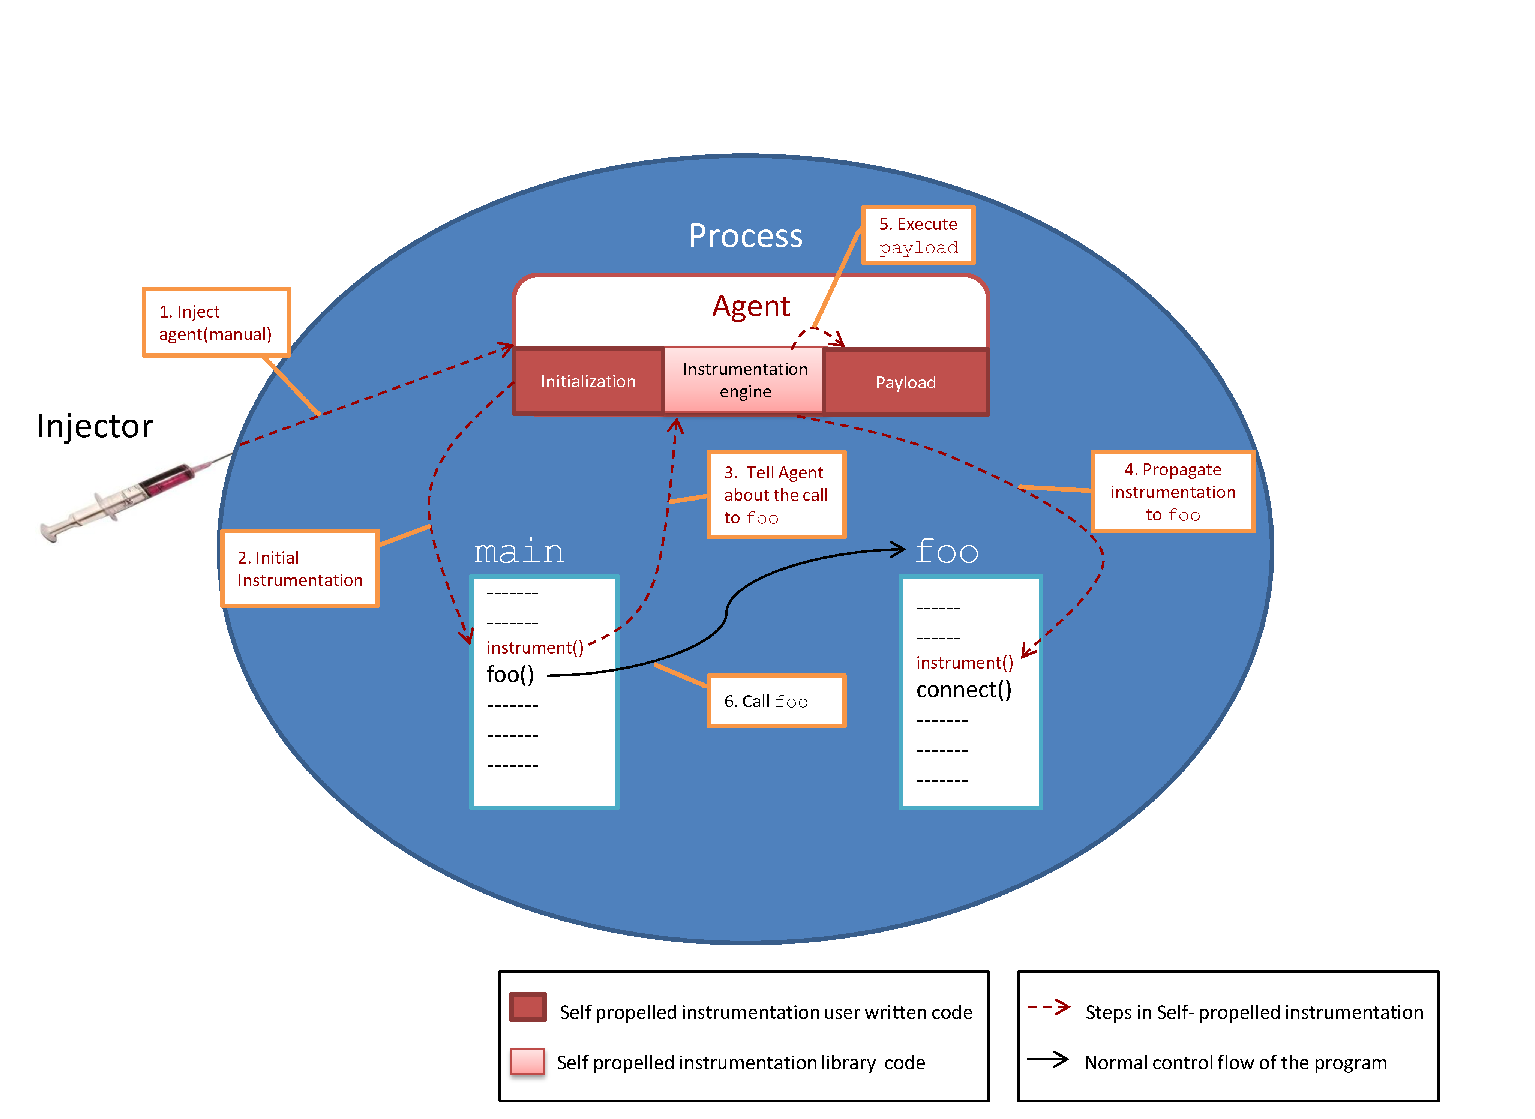
\includegraphics[width=0.90\textwidth]{figure/intraprocess.eps}
  \caption{Intra-process Self-propelled Instrumentation Workflow}
   \label{fig:Intra-process Self-propelled Instrumentation}
\end{figure}

Instrumenting all the function calls inside {\em main} function
internally calls the instrumentation engine, before each function
call. Instrumentation engine, in turn, propagates the instrumentation to
the called
function. If the called
function is within the same process, then instrumentation engine directly
propagates the instrumentation to the called function: i.e it instruments
all the function calls inside the called
function.  The instrumentation engine
also executes payload function either before instrumenting or after
instrumenting depending
on whether it is an entry payload or exit payload function. After the
instrumentation is done, the application's normal intra-process function
call execution
takes place. The workflow is visualized in Figure~\ref{fig:Intra-process
Self-propelled Instrumentation}.


\subsubsection{Inter-process propagation}
\begin{figure}[ht]
  \centering
  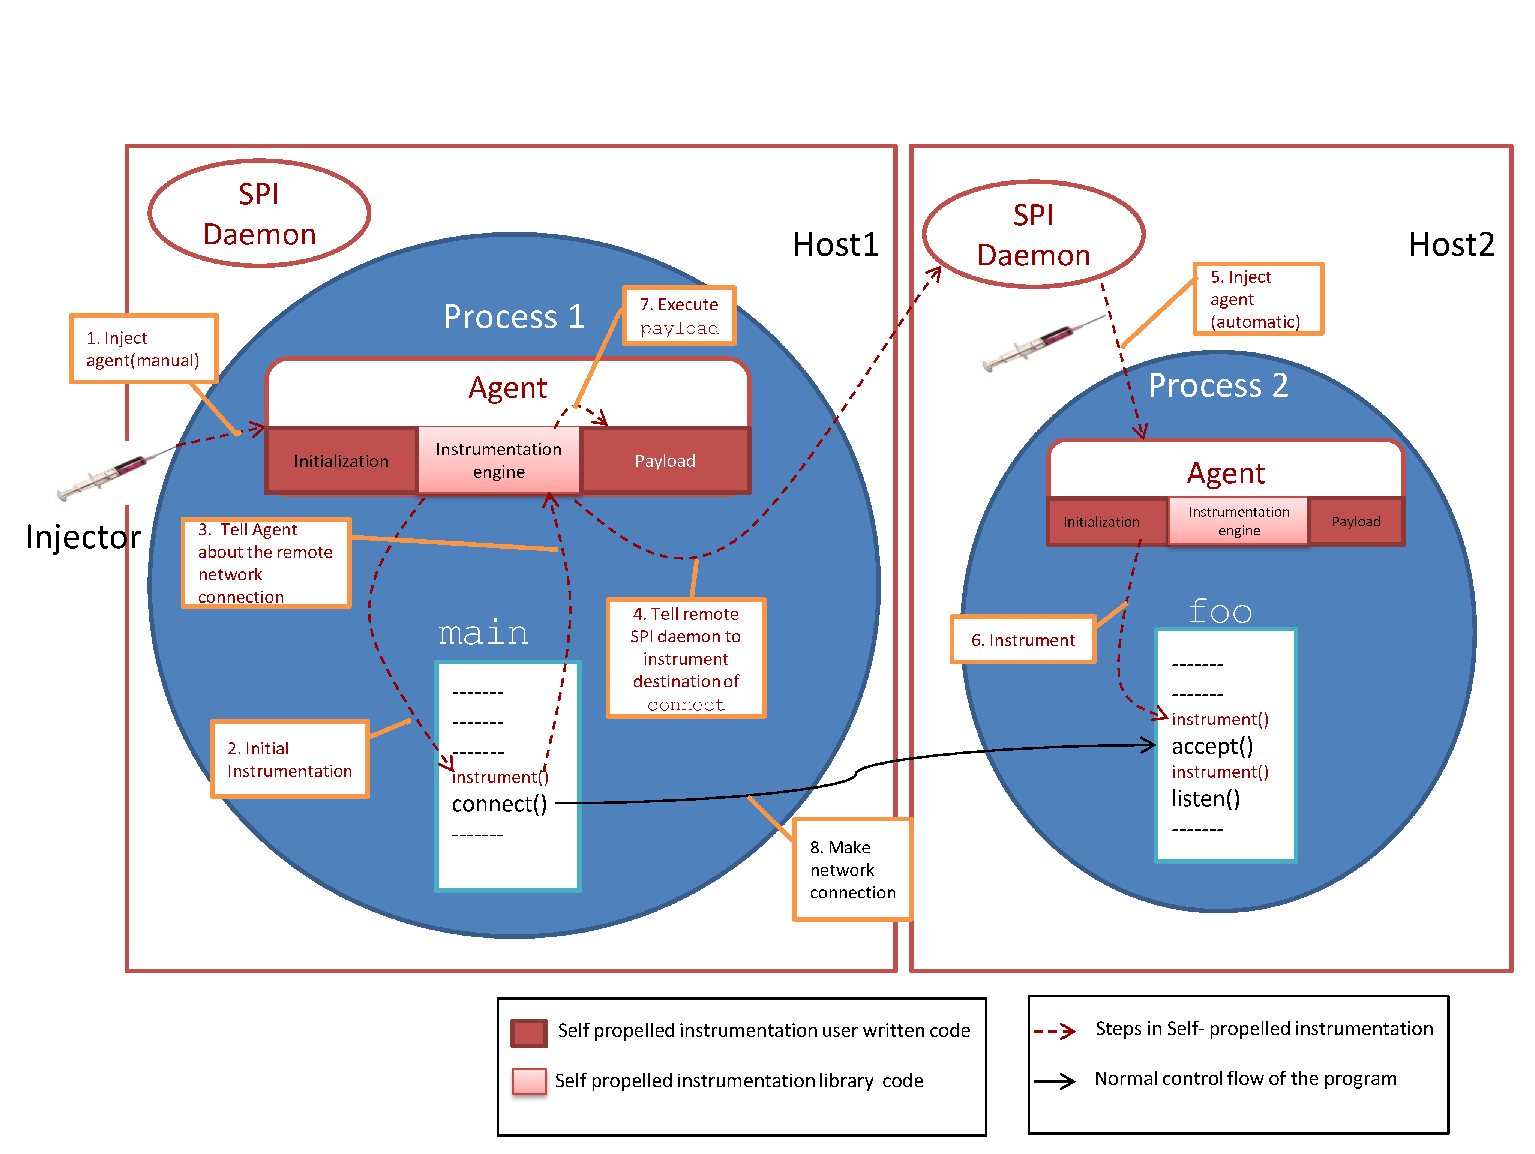
\includegraphics[width=0.90\textwidth]{figure/interprocess.eps}
  \caption{Inter-process Self-propelled Instrumentation Workflow}
  \label{fig:Inter-process Self-propelled Instrumentation}
\end{figure}

Similar to intra-process propagation, inter-process propagation also
instruments all the function calls inside an instrumenting function, but the
called function lies in a different process or host. So the instrumentation
engine, which gets called before every function call of the instrumenting
function, identifies that the called function is an inter-process function. It
then propagates the call to the SPI daemon of the appropriate host where
the called function is present.
The called SPI daemon then injects the agent shared library automatically
inside the process where the called function is located. Then the usual
process of \textit{initialisation} and \textit{initial instrumentation} goes
on inside the called function. After the instrumentation is done, the
application's normal inter-process function call execution takes place. In
the mean time, the instrumentation engine executes the payload depending on
whether it is an entry payload or an exit payload. The workflow is visualized
in Figure~\ref{fig:Inter-process Self-propelled Instrumentation}.





\section{Examples}
To illustrate the ideas of Self-propelled instrumentation, we present some
simple code examples that demonstrate how the API can be used.

\subsection{Writing Payload}
The primary task for users using self-propelled instrumentation is write
payload
functions that are invoked before or after each function call.
\lstset{language=[GNU]C++,basicstyle=\fontfamily{fvm}\selectfont\small}
\lstset{numbers=left}
\begin{lstlisting}[caption=Writing payload functions]
// Entry payload function that is invoked before each function call
void entry_payload(SpPoint* pt) {
  // Get function from point
  SpFunction* func = sp::Callee(pt);
  if (func == NULL) return;

  // If we encounter the system call exit, then print its argument
  if (func->name().compare("exit") == 0) {
    // Get argument
    sp::ArgumentHandle h;
    int* exit_code = (int*)sp::PopArgument(pt, &h, sizeof(int));
    printf("Exit Code: %d\n", *exit_code);
  }
  sp::Propel(pt);
}

// Exit payload function that is invoked after each function call
void exit_payload(SpPoint* pt) {
  // Get function from point
  SpFunction* func = sp::Callee(pt);
  if (func == NULL) return;

  // If we encounter the system call fork, then print its return value
  if (func->name().compare("fork") == 0) {
    pid_t child_pid = sp::ReturnValue(pt);
    // Print child process id from parent process side
    if (child_pid > 0) {
      printf("Child process id: %d\n", child_pid);
    }
  }
}
\end{lstlisting}
In the above code, we illustrate some common operations that users may want to
do in entry payload function or exit payload function.
Users can get CFG structures (e.g., function, block ...) from the argument {\em
  pt}.
Typically, there are some conditional branches to handle different functions,
e.g., handling exit and fork in the above code.
Users can also get arguments or return value for current function call.

\subsection{Configuration}
Users also need to provide the configuration code in the constructor
function of
the Agent shared library, which is mainly to register the user-provided payload
functions.
\lstset{language=[GNU]C++,basicstyle=\fontfamily{fvm}\selectfont\small}
\lstset{numbers=left}
\begin{lstlisting}[caption=Configuration code]
__attribute__((constructor))
void MyAgent() {
  sp::SpAgent::ptr agent = sp::SpAgent::Create();
  // Register entry payload function
  agent->SetInitEntry("entry_payload");
  // Register exit payload function
  agent->SetInitExit("exit_payload");
  // Initiate instrumentation
  agent->Go();
}
\end{lstlisting}
The above code shows the minimum operations needed to configure self-propelled
instrumentation.  The major things to do in the configuration code are to create
an Agent object that manages configurations, registers payload functions, and
initiates instrumentation.

\subsection{Using Injector}
The injector can be used to inject the agent shared library into a process. It
can also be injected to monitor all the processes running on a specific
port. The injector executable can be found inside $\$SP\_DIR/\$PLATFORM$. To
instrument a particular process with process id $pid$, use the following command

\apidesc{

./injector pid $pid$ LIB\_NAME

}

Similarly, to instrument all the processes running on a specific port,
use the following command

\apidesc{

./injector port $port$ LIB\_NAME

}



\subsection{Extending SPI}
This subsection discusses some code examples to extend self-propelled
instrumentation.
\subsubsection{Parser}
\lstset{language=[GNU]C++,basicstyle=\fontfamily{fvm}\selectfont\small}
\lstset{numbers=left}
\begin{lstlisting}[caption=Use customized parser]
// Extend SpParser and override the Parse() method to customize the parsing logic
class  MyParser : public SpParser {
  public:
    typedef SHARED_PTR(MyParser) ptr;
    AGENT_EXPORT static ptr Create() { return ptr(new MyParser); }
    AGENT_EXPORT virtual PatchAPI::PatchMgrPtr Parse() {
      // Implement your own parsing logic
    }
};

// Register the customized parser to self-propelled instrumentation
__attribute__((constructor))
void MyAgent() {
  sp::SpAgent::ptr agent = sp::SpAgent::Create();
  MyParser::ptr parser = MyParser::Create();
  agent->SetParser(parser);
  ...
}
\end{lstlisting}
The above code first extends SpParser to implement a customized parser for
parsing binary code into CFG structures. Developers mainly need to implement the
{\em Parse} method. Next, we register the customized parser in the agent library
by using {\em SpAgent::SetParser} method.

\subsubsection{Event}
\lstset{language=[GNU]C++,basicstyle=\fontfamily{fvm}\selectfont\small}
\lstset{numbers=left}
\begin{lstlisting}[caption=Use customized event]
// Extend SpEvent and override the RegisterEvent() method to do 
// initial instrumentation
class  MyEvent : public SpEvent {
  public:
    typedef SHARED_PTR(MyEvent) ptr;
    static ptr Create() { return ptr(new MyEvent()); }
    virtual void RegisterEvent() {}
};

// Register the customized event to self-propelled instrumentation
__attribute__((constructor))
void MyAgent() {
  sp::SpAgent::ptr agent = sp::SpAgent::Create();
  MyEvent::ptr event = MyEvent::Create();
  agent->SetInitEvent(event);
  ...
}
\end{lstlisting}
The above code first extends SpEvent to implement the {\em RegisterEvent} method
that does initial instrumentation. Next, we register the customized event in
the agent library by using {\em SpAgent::SetInitEvent} method.

\subsubsection{Instrumentation Workers}
\lstset{language=[GNU]C++,basicstyle=\fontfamily{fvm}\selectfont\small}
\lstset{numbers=left}
\begin{lstlisting}[caption=Use customized instrumentation worker]
// Extend InstWorkerDelegate to build a customized instrumentation worker
class MyInstWorker : public InstWorkerDelegate {
  public:
		// Instrument a point
    virtual bool run(SpPoint* pt) {}

		// Uninstrument a point
		virtual bool undo(SpPoint* pt) {}

		// Save code that will be modified for a point
		virtual bool save(SpPoint* pt) {}

		// How to install instrumentation?
		virtual InstallMethod install_method() {}
};

// Register MyInstWorker in the instrumenter
SpInstrumenter::SpInstrumenter(ph::AddrSpace* as) {
  ...
	workers_.push_back(new SpringboardWorker);
	workers_.push_back(new TrapWorker);
	workers_.push_back(new MyInstWorker);
  ...
}
\end{lstlisting}


\subsubsection{IPC Workers}
\lstset{language=[GNU]C++,basicstyle=\fontfamily{fvm}\selectfont\small}
\lstset{numbers=left}
\begin{lstlisting}[caption=Use customized IPC worker]
class  MyIpcWorker : public SpIpcWorkerDelegate {
  public:
    virtual void SetRemoteStartTracing(char yes_or_no,
                                       SpChannel* c) {}
    virtual void SetLocalStartTracing(char yes_or_no) {}
    virtual char CanStartTracing(int fd) {}
    virtual bool Inject(SpChannel*, char* agent_path = NULL) {}
    virtual SpChannel* GetChannel(int fd,
                                  ChannelRW rw,
                                  void* arg = NULL) {}
    virtual void CloseChannel(int fd) {}
};

// Register MyIpcWorker to self-propelled instrumentation
SpIpcMgr::SpIpcMgr() {
  ...
  pipe_worker_ = new SpPipeWorker;
  worker_set_.insert(pipe_worker_);

  tcp_worker_ = new SpTcpWorker;
  worker_set_.insert(tcp_worker_);
  
  my_ipc_worker_ = new MyIpcWorker;
  worker_set_.insert(my_ipc_worker_);
  ...
}
\end{lstlisting}

\section{Class Reference}

% In both user and developer manual
\subsection{Public Interface}
\subsubsection{Class Agent}
\textbf{Declared in}: src/agent/agent.h

\begin{apient}
void SetInitEntry(string);
\end{apient}
\apidesc{

Sets the entry payload function name. By default, the entry payload function is
``default_entry'', which simply prints out all executed functions' name.

}

\begin{apient}
void SetInitExit(string);
\end{apient}
\apidesc{

Sets the exit payload function name. By default, there is not exit payload
function.

}

\begin{apient}
void SetLibrariesToInstrument(const StringSet& libs);
\end{apient}
\apidesc{

Sets the set of names of libraries loaded in the application process that will
be instrumented. By default, we only instrument the executable binary code and
don't instrument loaded shared libraries.

}

\begin{apient}
void SetFuncsNotToInstrument(const StringSet& funcs);
\end{apient}
\apidesc{
Sets the set of names of functions in the application process that will
NOT be instrumented. By default, we instrument all functions.
}

\begin{apient}
void EnableParseOnly(const bool yes_or_no);
\end{apient}
\apidesc{

Enables or disables ParseOnly option. If yes\_or\_no is true, then after parsing
the binary code, we don't do instrumentation; otherwise, instrumentation is
conducted after parsing. By default, ParseOnly option is disabled.

}

\begin{apient}
void EnableIpc(const bool yes_or_no);
\end{apient}
\apidesc{

Enable or disable inter-process instrumentation propagation. By default,
inter-process instrumentation propagation is disabled.

}

\begin{apient}
void EnableHandleDlopen(const bool yes_or_no);
\end{apient}
\apidesc{

Enable or disable propagating instrumentation to library loaded via dlopen. By
default, it is disabled.

}

\begin{apient}
void EnableMultithread(const bool yes_or_no);
\end{apient}
\apidesc{

Enable or disable propagating instrumentation across thread. By default, it is
disabled.

}

\begin{apient}
void Go();
\end{apient}
\apidesc{

Starts initial instrumentation.

}

\subsubsection{Class SpPoint}
\textbf{Declared in}: src/agent/patchapi/point.h

\begin{apient}
bool tailcall();
\end{apient}
\apidesc{

Indicates whether or not the function call at this point is a tail call.

}

\begin{apient}
SpBlock* GetBlock() const;
\end{apient}
\apidesc{

Returns the call block at this point.

}

\begin{apient}
SpObject* GetObject() const;
\end{apient}
\apidesc{
Returns the binary object at this point.
}


\subsubsection{Class SpObject}
\textbf{Declared in}: src/agent/patchapi/object.h

\begin{apient}
std::string name() const;
\end{apient}
\apidesc{
Returns the binary object's name.
}

This class inherits PatchAPI::PatchObject. Please refer to PatchAPI document for
the complete list of methods.

\subsubsection{Class SpFunction}
\textbf{Declared in}: src/agent/patchapi/cfg.h

\begin{apient}
SpObject* GetObject() const;
\end{apient}
\apidesc{
Returns the binary object containing this function.
}

\begin{apient}
std::string GetMangledName();
\end{apient}
\apidesc{
Returns the mangled name of this function.
}

\begin{apient}
std::string GetPrettyName();
\end{apient}
\apidesc{
Returns the demangled name of this function.
}

\begin{apient}
std::string name();
\end{apient}
\apidesc{
Returns the demangled name of this function, the same as calling GetPrettyName().
}

This class inherits PatchAPI::PatchFunction. Please refer to PatchAPI document
for the complete list of methods.

\subsubsection{Class SpBlock}
\textbf{Declared in}: src/agent/patchapi/cfg.h

\begin{apient}
SpObject* GetObject() const;
\end{apient}
\apidesc{
Returns the binary object containing this block.
}

\begin{apient}
in::Instruction::Ptr orig_call_insn() const;
\end{apient}
\apidesc{

Returns an InstructionAPI::Instruction instance of the call instruction in this
block.

}

This class inherits PatchAPI::PatchBlock. Please refer to PatchAPI document for
the complete list of methods.

\subsubsection{Class SpEdge}
\textbf{Declared in}: src/agent/patchapi/cfg.h

This class inherits PatchAPI::PatchEdge. Please refer to PatchAPI document for
the complete list of methods.

\subsubsection{Utility Functions}
\textbf{Declared in}: src/agent/payload.h

Utility functions are used when writing payload functions.

\begin{apient}
SpFunction* Callee(SpPoint* pt);
\end{apient}
\apidesc{
Returns an instance of SpFunction for current function call. 
The argument \emph{pt} represents the instrumentation point for current function
call.
If it fails, it returns NULL.
}

\begin{apient}
bool IsInstrumentable(SpPoint* pt);
\end{apient}
\apidesc{
Indicates whether or not the point is instrumentable.
}

\begin{apient}
void Propel(SpPoint* pt);
\end{apient}
\apidesc{

Propagates instrumentation to callees of the function called at the specified
point {\em pt}.

}

\begin{apient}
bool IsIpcWrite(SpPoint* pt); 
bool IsIpcRead(SpPoint* pt); 
\end{apient}
\apidesc{

Indicates whether or not the function called at the specified point is a
inter-process communication write / read function.

}

\begin{apient}
struct ArgumentHandle;
void* PopArgument(SpPoint* pt,
                  ArgumentHandle* h,
                  size_t size);
\end{apient}
\apidesc{

Gets a pointer to an argument of the function call at the specified point {\em
  pt}.
All arguments passed to the function call are in a stack associated with the
ArgumentHandle structure {\em h}. 
Leftmost argument is at the top of the stack.
The {\em size} parameter specifies the size of the argument that is about to be
popped.

}

\begin{apient}
long ReturnValue(SpPoint* pt);
\end{apient}
\apidesc{
Returns the return value of the function call at the specified point {\em pt}.
}

% In developer manual only
\subsection{Private Interface}
\subsubsection{Class SpParser}
\textbf{Declared in}: src/agent/parser.h

\begin{apient}
static ptr Create();
\end{apient}
\apidesc{
}

\begin{apient}
SpObject* exe() const;
\end{apient}
\apidesc{
Returns the executable's binary object.
}

\begin{apient}
PatchAPI::PatchMgrPtr Parse();
\end{apient}
\apidesc{
}

\begin{apient}
PatchAPI::PatchMgrPtr Parse();
\end{apient}
\apidesc{
}

\begin{apient}
string agent_name()
\end{apient}
\apidesc{
}

\begin{apient}
bool injected()
\end{apient}
\apidesc{
}

\begin{apient}
void GetFrame(long* pc, long* sp, long* bp)
\end{apient}
\apidesc{
}

\begin{apient}
SpFunction* FindFunction(dt::Address absolute_addr);
\end{apient}
\apidesc{
}

\begin{apient}
SpFunction* FindFunction(string func_name_without_path);
\end{apient}
\apidesc{
}

\begin{apient}
bool FindFunction(string func_name_without_path, FuncSet* found_funcs);
\end{apient}
\apidesc{
}

\begin{apient}
SpFunction* callee(SpPoint* point, bool parse_indirect = false);
\end{apient}
\apidesc{
}

\begin{apient}
string DumpInsns(void* addr, size_t size);
\end{apient}
\apidesc{
}

\begin{apient}
static bool ParseDlExit(SpPoint* pt);
\end{apient}
\apidesc{
}

\subsubsection{Class SpContext}
\textbf{Declared in}: src/agent/context.h

\begin{apient}
static SpContext* Create();
\end{apient}
\apidesc{
}

\begin{apient}
string init_entry_name() const
\end{apient}
\apidesc{
}

\begin{apient}
string init_exit_name() const
\end{apient}
\apidesc{
}

\begin{apient}
void GetCallStack(FuncSet* func_set);
\end{apient}
\apidesc{
}

\begin{apient}
void GetCallStack(FuncSet* func_set);
\end{apient}
\apidesc{
}

\begin{apient}
bool IsMultithreadEnabled() const;
\end{apient}
\apidesc{
}

\begin{apient}
bool IsHandleDlopenEnabled() const;
\end{apient}
\apidesc{
}

\begin{apient}
bool IsDirectcallOnlyEnabled() const;
\end{apient}
\apidesc{
}

\begin{apient}
SpPropeller::ptr init_propeller() const;
\end{apient}
\apidesc{
}

\begin{apient}
PayloadFunc init_entry() const;
PayloadFunc init_exit() const;
\end{apient}
\apidesc{
}

\begin{apient}
PayloadFunc wrapper_exit() const;
PayloadFunc wrapper_entry() const;
\end{apient}
\apidesc{
}

\subsubsection{Class SpEvent}
\textbf{Declared in}: src/agent/event.h

\begin{apient}
static ptr Create();
\end{apient}
\apidesc{
}

\begin{apient}
virtual void RegisterEvent();
\end{apient}
\apidesc{
}

\subsubsection{Class AsyncEvent}
\textbf{Declared in}: src/agent/event.h

\begin{apient}
static ptr Create(int signum = SIGALRM,
                  int sec = 5);
\end{apient}
\apidesc{
}

\subsubsection{Class SyncEvent}
\textbf{Declared in}: src/agent/event.h

\begin{apient}
static ptr Create();
\end{apient}
\apidesc{
}

\subsubsection{Class FuncEvent}
\textbf{Declared in}: src/agent/event.h

\begin{apient}
static ptr Create(StringSet& funcs);
\end{apient}
\apidesc{
}

\subsubsection{Class CallEvent}
\textbf{Declared in}: src/agent/event.h

\begin{apient}
static ptr Create(StringSet& funcs);
\end{apient}
\apidesc{
}

\subsubsection{Class CombEvent}
\textbf{Declared in}: src/agent/event.h

\begin{apient}
static ptr Create(EventSet& events);
\end{apient}
\apidesc{
}

\subsubsection{Class SpPropeller}
\textbf{Declared in}: src/agent/propeller.h

\begin{apient}
static ptr Create();
\end{apient}
\apidesc{
}

\begin{apient}
bool go(SpFunction* func,
        PayloadFunc entry,
        PayloadFunc exit,
        SpPoint* pt = NULL,
        StringSet* inst_calls = NULL);
\end{apient}
\apidesc{
}

\subsubsection{Class SpSnippet}
\textbf{Declared in}: src/agent/snippet.h

\begin{apient}
static ptr create(SpFunction* f,
                  SpPoint* pt,
                  PayloadFunc entry,
                  PayloadFunc exit);
\end{apient}
\apidesc{
}

\begin{apient}
char* BuildBlob(const size_t est_size,
                const bool reloc = false);
\end{apient}
\apidesc{
}

\begin{apient}
size_t GetBlobSize() const;
\end{apient}
\apidesc{
}

\begin{apient}
SpBlock* FindSpringboard();
\end{apient}
\apidesc{
}

\begin{apient}
char* RelocateSpring(SpBlock* spring_blk);
\end{apient}
\apidesc{
}

\begin{apient}
size_t GetRelocSpringSize() const;
\end{apient}
\apidesc{
}

\begin{apient}
dt::Address GetSavedReg(dt::MachRegister reg);
\end{apient}
\apidesc{
}

\begin{apient}
long GetRetVal();
\end{apient}
\apidesc{
}

\begin{apient}
void* PopArgument(ArgumentHandle* h, size_t size);
\end{apient}
\apidesc{
}

\begin{apient}
PayloadFunc entry() const;
\end{apient}
\apidesc{
}

\begin{apient}
PayloadFunc exit() const;
\end{apient}
\apidesc{
}

\begin{apient}
SpPoint* point() const;
\end{apient}
\apidesc{
}


\subsubsection{Class SpAddrSpace}
\textbf{Declared in}: src/agent/patchapi/addr\_space.h

\begin{apient}
bool SetMemoryPermission(dt::Address addr,
                         size_t length,
                         int perm);
\end{apient}
\apidesc{
}

\begin{apient}
void InitMemoryAllocator();
\end{apient}
\apidesc{
}

\subsubsection{Inst Workers}

\textbf{Class InstWorkerDelegate}

\textbf{Declared in}: src/agent/inst\_workers/inst_worker_delegate.h

\begin{apient}
virtual bool run(SpPoint* pt);
\end{apient}
\apidesc{
Instrument a point.
}

\begin{apient}
virtual bool undo(SpPoint* pt);
\end{apient}
\apidesc{
Uninstrument a point.
}

\begin{apient}
virtual bool save(SpPoint* pt);
\end{apient}
\apidesc{
Save code that will be modified for a point.
}

\begin{apient}
virtual InstallMethod install_method() const;
\end{apient}
\apidesc{
Returns the method of instrumentation installation.
}

\textbf{Class RelocCallInsnWorker}

\textbf{Declared in}: src/agent/inst\_workers/callinsn_worker_impl.h

\textbf{Class RelocCallBlockWorker}

\textbf{Declared in}: src/agent/inst\_workers/callblk_worker_impl.h

\textbf{Class SpringboardWorker}

\textbf{Declared in}: src/agent/inst\_workers/spring_worker_impl.h

\textbf{Class TrapWorker}

\textbf{Declared in}: src/agent/inst\_workers/trap_worker_impl.h


\subsubsection{Class SpThreadMgr}
\textbf{Declared in}: src/agent/thread\_mgr.h

\begin{apient}
static bool BeforeEntry(SpPoint*);
\end{apient}
\apidesc{
}

\subsubsection{Class IpcMgr}
\textbf{Declared in}: src/agent/ipc/ipc\_mgr.h

\begin{apient}
SpChannel* GetChannel(int fd,
                      ChannelRW rw);
\end{apient}
\apidesc{
}

\begin{apient}
SpIpcWorkerDelegate* GetWorker(int fd);
\end{apient}
\apidesc{
}

\begin{apient}
void GetWriteParam(SpPoint* pt,
                   int* fd_out,
                   void** buf_out,
                   char* c_out,
                   size_t* size_out,
                   sockaddr** sa_out);
\end{apient}
\apidesc{
}

\begin{apient}
void GetReadParam(SpPoint* pt,
                  int* fd_out,
                  void** buf_out,
                  size_t* size_out);
\end{apient}
\apidesc{
}

\begin{apient}
bool is_fork(const char* f);
\end{apient}
\apidesc{
}

\begin{apient}
bool is_popen(const char* f);
\end{apient}
\apidesc{
}

\begin{apient}
char start_tracing(int fd);
\end{apient}
\apidesc{
}

\begin{apient}
static bool BeforeEntry(SpPoint*);
\end{apient}
\apidesc{
}

\begin{apient}
static bool BeforeExit(SpPoint*);
\end{apient}
\apidesc{
}

\begin{apient}
SpPipeWorker* pipe_worker() const;
\end{apient}
\apidesc{
}

\begin{apient}
SpTcpWorker* tcp_worker() const;
\end{apient}
\apidesc{
}

\begin{apient}
SpUdpWorker* udp_worker() const;
\end{apient}
\apidesc{
}

\subsubsection{Class SpChannel}
\textbf{Declared in}: src/agent/ipc/channel.h

\subsubsection{IPC Workers}
\textbf{Declared in}: src/agent/ipc/ipc\_workers/

\textbf{Class SpIpcWorkerDelegate}

\textbf{Declared in}: src/agent/ipc/ipc\_workers/ipc\_worker\_delegate.h

\begin{apient}
virtual void SetStartTracing(char yes_or_no,
                             SpChannel* c);
\end{apient}
\apidesc{
}

\begin{apient}
virtual void SetStartTracing(char yes_or_no);
\end{apient}
\apidesc{
}

\begin{apient}
virtual char start_tracing(int fd);
\end{apient}
\apidesc{
}

\begin{apient}
virtual bool Inject(SpChannel*, char* agent_path = NULL);
\end{apient}
\apidesc{
}

\begin{apient}
virtual SpChannel* GetChannel(int fd,
                              ChannelRW rw,
                              void* arg = NULL);
\end{apient}
\apidesc{
}

\textbf{Class SpPipeWorker}

\textbf{Declared in}: src/agent/ipc/ipc\_workers/pipe\_worker\_impl.h

\textbf{Class SpTcpWorker}

\textbf{Declared in}: src/agent/ipc/ipc\_workers/tcp\_worker\_impl.h

\textbf{Class SpUdpWorker}

\textbf{Declared in}: src/agent/ipc/ipc\_workers/udp\_worker\_impl.h


\appendix
\section{Installation}
This appendix describes how to build SecSTAR from source code, which can be downloaded from \url{http://www.paradyn.org} or \url{http://www.dyninst.org}. \\

\textbf \underline{BUILDING ON UNIX}\\
Before starting to build SecSTAR, you have to make sure that you have already installed and built Dyninst. (refer http://www.dyninst.org/sites/default/files/manuals/dyninst/dyninstProgGuide.pdf - Appendix D for building Dyninst) \\

Building SecSTAR on UNIX platforms is a very simple three step process that involves: unpacking the SecSTAR source, configuring paths in config.mk, and running the build. \\

\textbf{1. Unpacking the SecSTAR source:} \\
SecSTAR’s source code is packaged in a -----(tar.gz) format. If your SecSTAR source tarball is called \textit{src\_SecSTAR.tar.gz}, then you could extract it with the commands \textit{gunzip src\_SecSTAR.tar.gz ; tar –xvf src\_SecSTAR.tar}. This will create a list of directories and files.  \\

\textbf{2. Configuring paths in config.mk} \\
After unpacking,the next thing is to set DYNINST\_ROOT, PLATFORM, and LD\_LIBRARY\_PATH environment variables in.  \\
{\textit DYNINST\_ROOT} should be set to path of the directory that contains subdirectories like dyninstAPI, parse API etc.,  i.e. within dyninst directory SP\_DIR should be set to the the path of the current working directory (where self propelled instrumentation is installed). \\

\$DYNLINK should be set true for building agent as a small shared library that relies on other shared libraries. Otherwise, a single huge shared library that static-linked all libraries(doubt) \\

\$PLATFORM should be set to one of the following values depending upon what operating system you are running on: \\
\begin{itemize}
  \item i386-unknown-linux 2.4: Linux 2.4/2.6 on an Intel x86 processor
  \item x86\_64-unknown-linux2.4: Linux 2.4/2.6 on an AMD-64/Intel x86-64 processor
\end{itemize}

Before building, you should also check whether \$LD\_LIBRARY\_PATH variable is set. If you are using bash shell, then open ~/.bashrc file and check if \$LD\_LIBRARY\_PATH is already present. If not, then LD\_LIBRARY\_PATH variable should be set in a way that it includes  \${DYNINST\_LIB PATH} directories.  If you are using C shell, then do the above mentioned tasks in ~/.cshrc file. \\
 
\textbf{3. Building SecSTAR:} \\
Once config.mk is set, you are ready to build SecSTAR. Move to \$PLATFORM directory  and execute the command \textit{make}. This will build ------(Dyninst’s mutator library, the Dyninst runtime library, and Dyninst’s test suite). ---- (Successfully built binaries will be stored in a directory named after your platform at the same level as the dyninst directory) \\


\section{Testing}
\section{Directory Organization}

\bibliographystyle{abbrv}
\bibliography{ref}

\end{document}
